\documentclass[12pt,a4paper]{article}
\usepackage{amsmath}
\usepackage{mathtext}
\usepackage{icomma}
\usepackage{amsfonts}
\usepackage{amssymb}
\usepackage[utf8]{inputenc}
\usepackage[T1,T2A]{fontenc}
\usepackage[english, russian]{babel}
\usepackage{graphicx}
\usepackage[left=2cm,right=2cm,top=2cm,bottom=2cm]{geometry}
\usepackage{calc}
\usepackage{wrapfig}
\usepackage{setspace}
\usepackage{indentfirst}
\usepackage{subfigure}
\usepackage[table,xcdraw]{xcolor}


\title{
Отчет о выполнении лабораторной работы 2.1.3 \\
Определение $C_p/C_\upsilon$ по скорости звука в газе
}

\author{Исламов Сардор, группа Б02-111}
\date{31 января 2022 г. }

\begin{document}
\maketitle

\subparagraph*{Аннотация.}

В работе измерены частота и длина волны при резонансе звуковых колебаний в газе, заполянющем трубу. Также с помощью уравнения состояния идеального газа определен показатель адиабаты.

\subsection*{Теоретические сведения}

Один из наиболее точных методов измерения показателя адиабаты $\gamma$ основан на зависимости от него скорости распространения звуковой волны в газе. Последняя в газах определяется формулой $c = \sqrt{\frac{\gamma RT}{\mu}}$, из которой можно выразить показатель адиабаты:
 	\begin{equation}
 	\gamma = \frac{\mu}{RT}c^2,
 	\end{equation}
где $T$ --- температура газа, $\mu$ --- его молярная масса, а $R$ --- газовая постоянная. \\
Скорость $c$ звука связана с его частотой $f$ и длиной волны $\lambda$ соотношением
	\begin{equation}
	c = \lambda f.
	\end{equation}
С волнами в трубке удобнее всего работать при резонансе. Условие резонанса выглядит как
	\begin{equation}
	L = n\frac{\lambda}{2},
	\end{equation}
где $L$ --- длина трубки, $\lambda$ --- длина волны, $n$ --- целое число.\\
Подбор условий резонанса можно поризвести двояко:

1. При неизменной частоте $f$ генератора можно изменять длину трубы $L$, резонанс легко заметить при резком увеличении амплитуды колебаний на осциллографе. Для последовательных резонансов имеем

\begin{equation*}
    L_1 = \frac \lambda 2 ,\ L_{2} = 2 \frac \lambda 2,\ ...,\ L_n = n \frac{\lambda}{2},
\end{equation*}
таким образом $\lambda/2$ равно угловому коэффициенту графика зависимости длины трубы $L$ от номера резонанса $k$.

2. При постоянной длине трубки изменяется частота звуковых колебаний $f$, а с ней и длина звуковой волны $\lambda$. Для последовательных резонансов можно записать
	\begin{equation*}
	L = n\frac{\lambda_1}{2} = (n + 1)\frac{\lambda_2}{2} = ... = (n + k)\frac{\lambda_{k + 1}}{2},
	\end{equation*}

С учётом (2) имеем
	\begin{equation}
	f_{t+1} = \frac{c}{\lambda_{t+1}} = f_1 + \frac{c}{2L}t~ (t = 0, 1,..., k)
	\end{equation}
Таким образом, $c/2L$ можно найти как угловой коэффициент графика зависимости частоты от номера резонанса.

\subsection*{Экспериментальные методы}

\subparagraph{В работе используются:} звуковой генератор ГЗ; электорнный осциллограф ЭО; микрофон; телефон; раздвижная труба; теплоизолированная труба, обогреваемая водой из термостата; баллон со сжатым углекислым газом; газгольдер.

 Схема установки, используемой в первом случае приведена на рис. 1.
	\begin{figure}[htp]
		\centering
		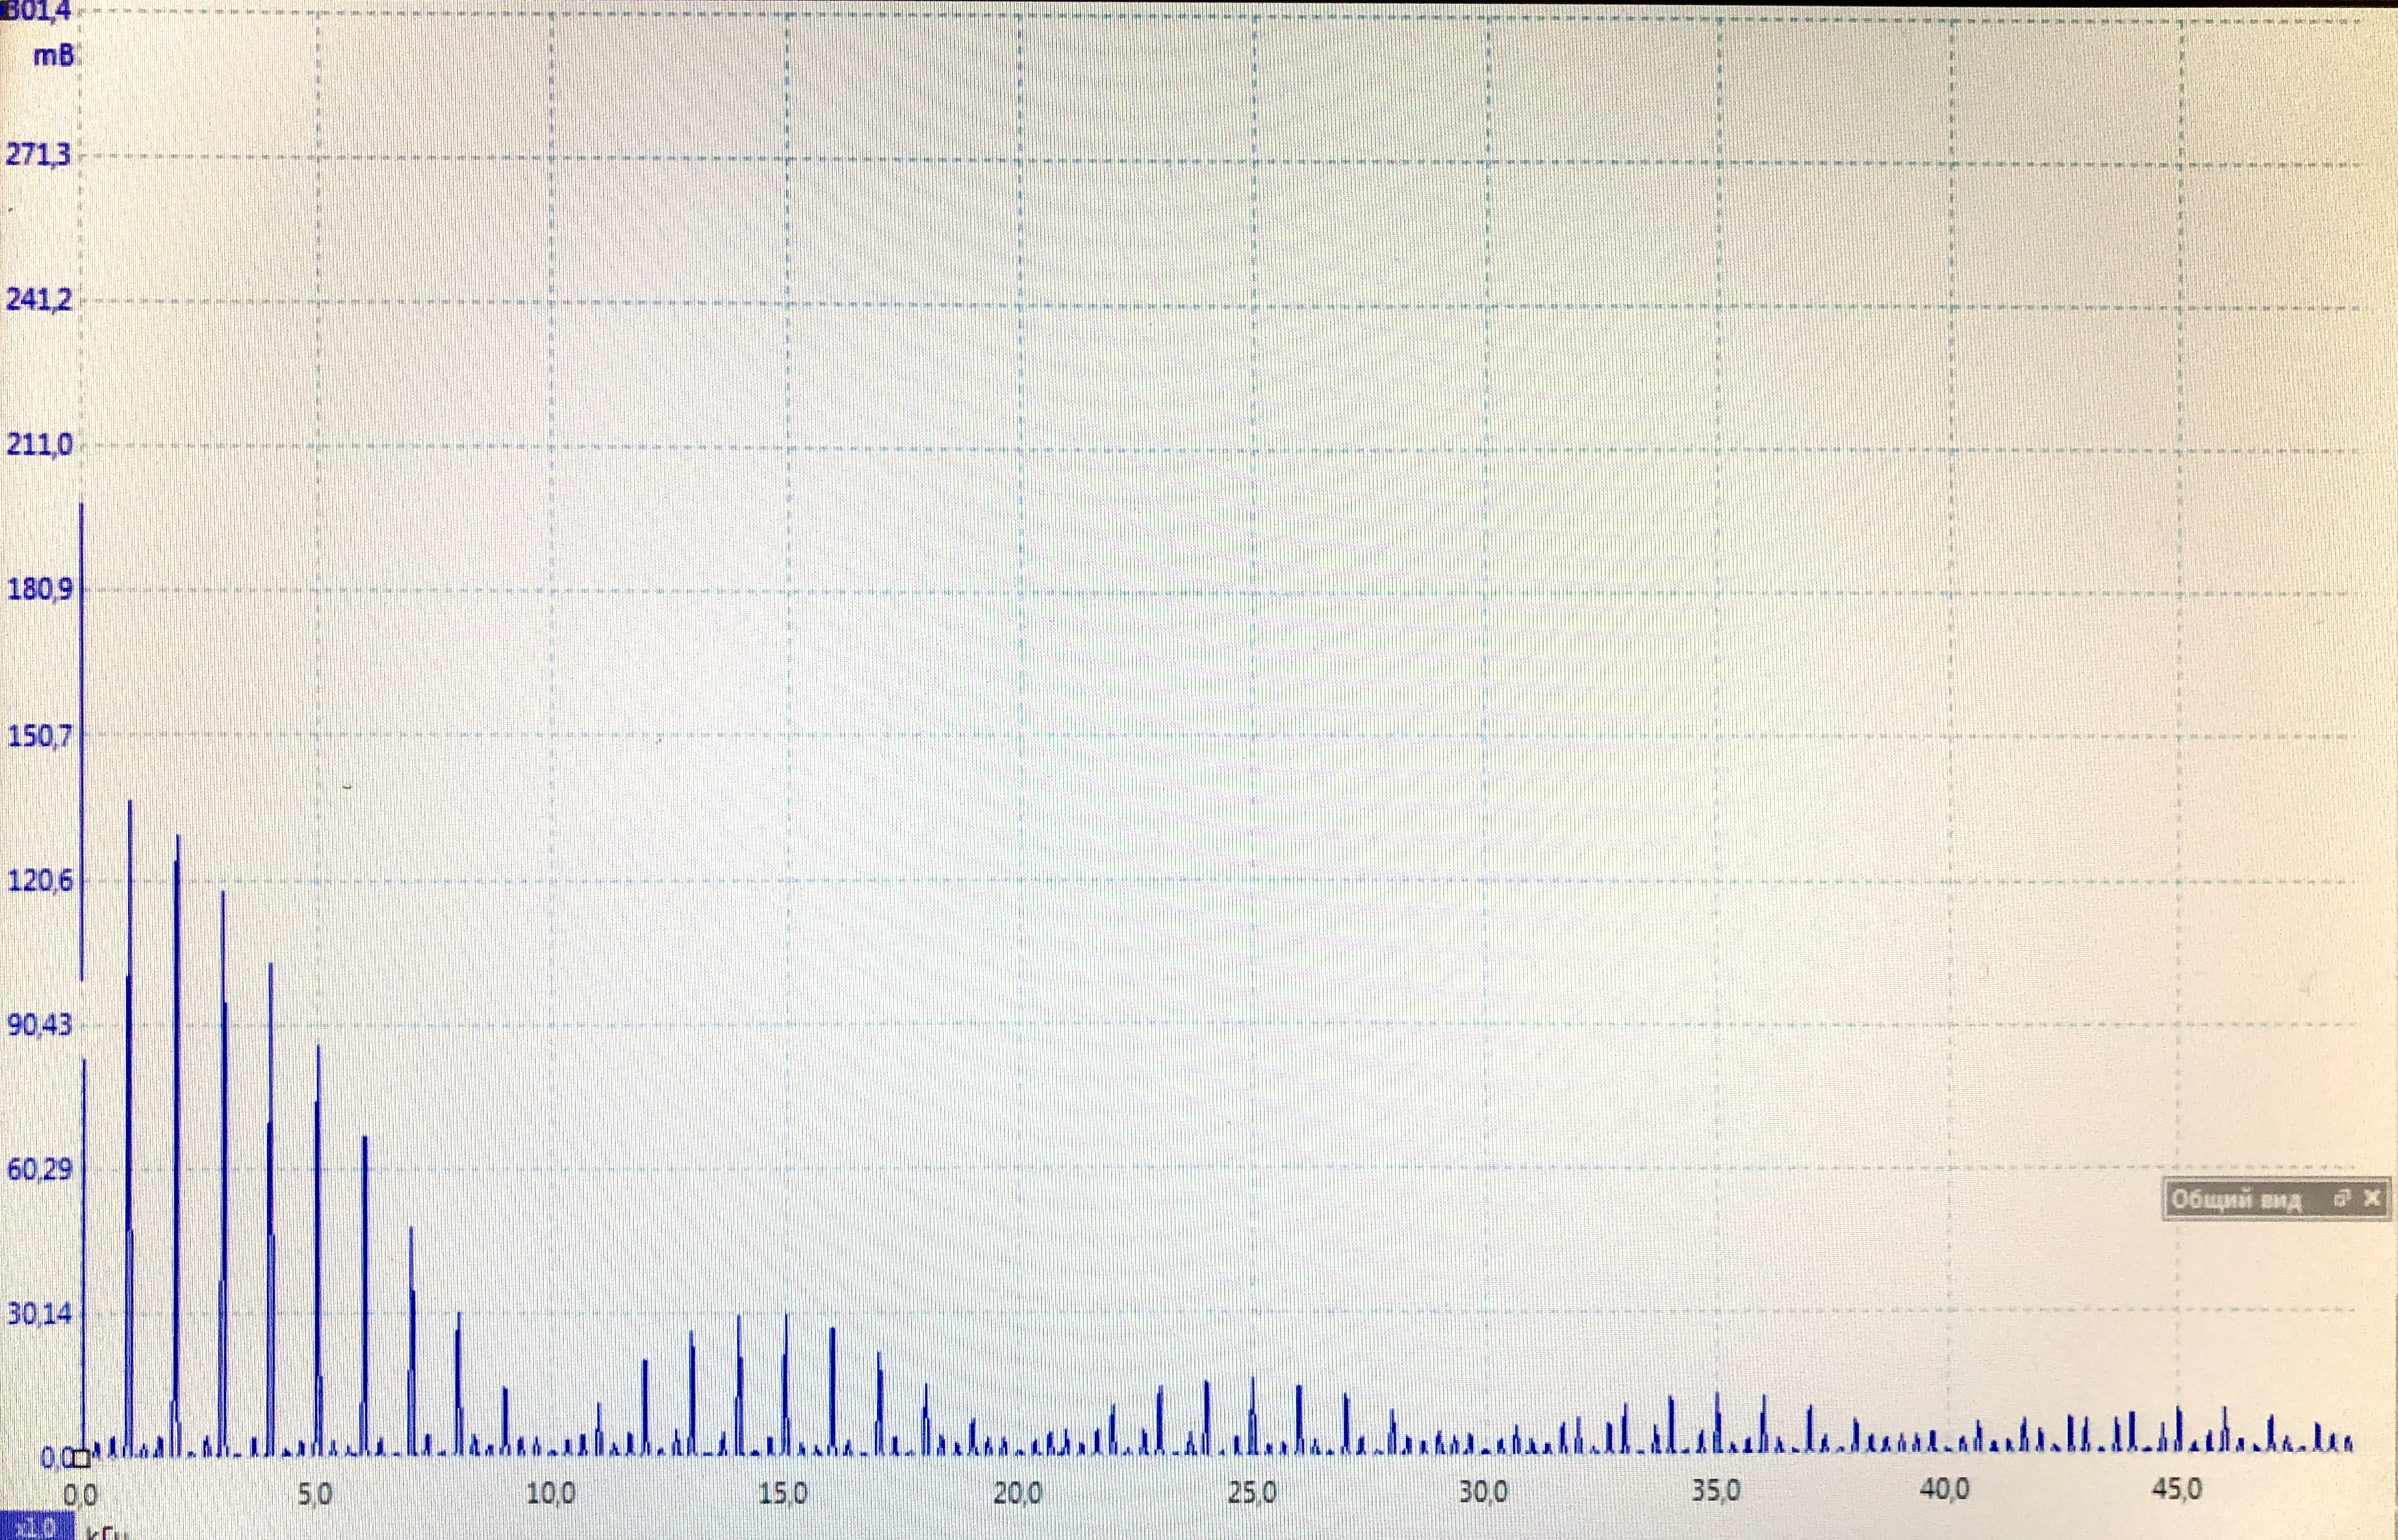
\includegraphics[width=0.5\linewidth]{2.png}
		\caption{Схема установки для измерения скорости звука при помощи раздвижной трубы}
	\end{figure}
	
 Схема установки, используемой во втором случае приведена на рис. 2.
	\begin{figure}[htp]
		\centering
		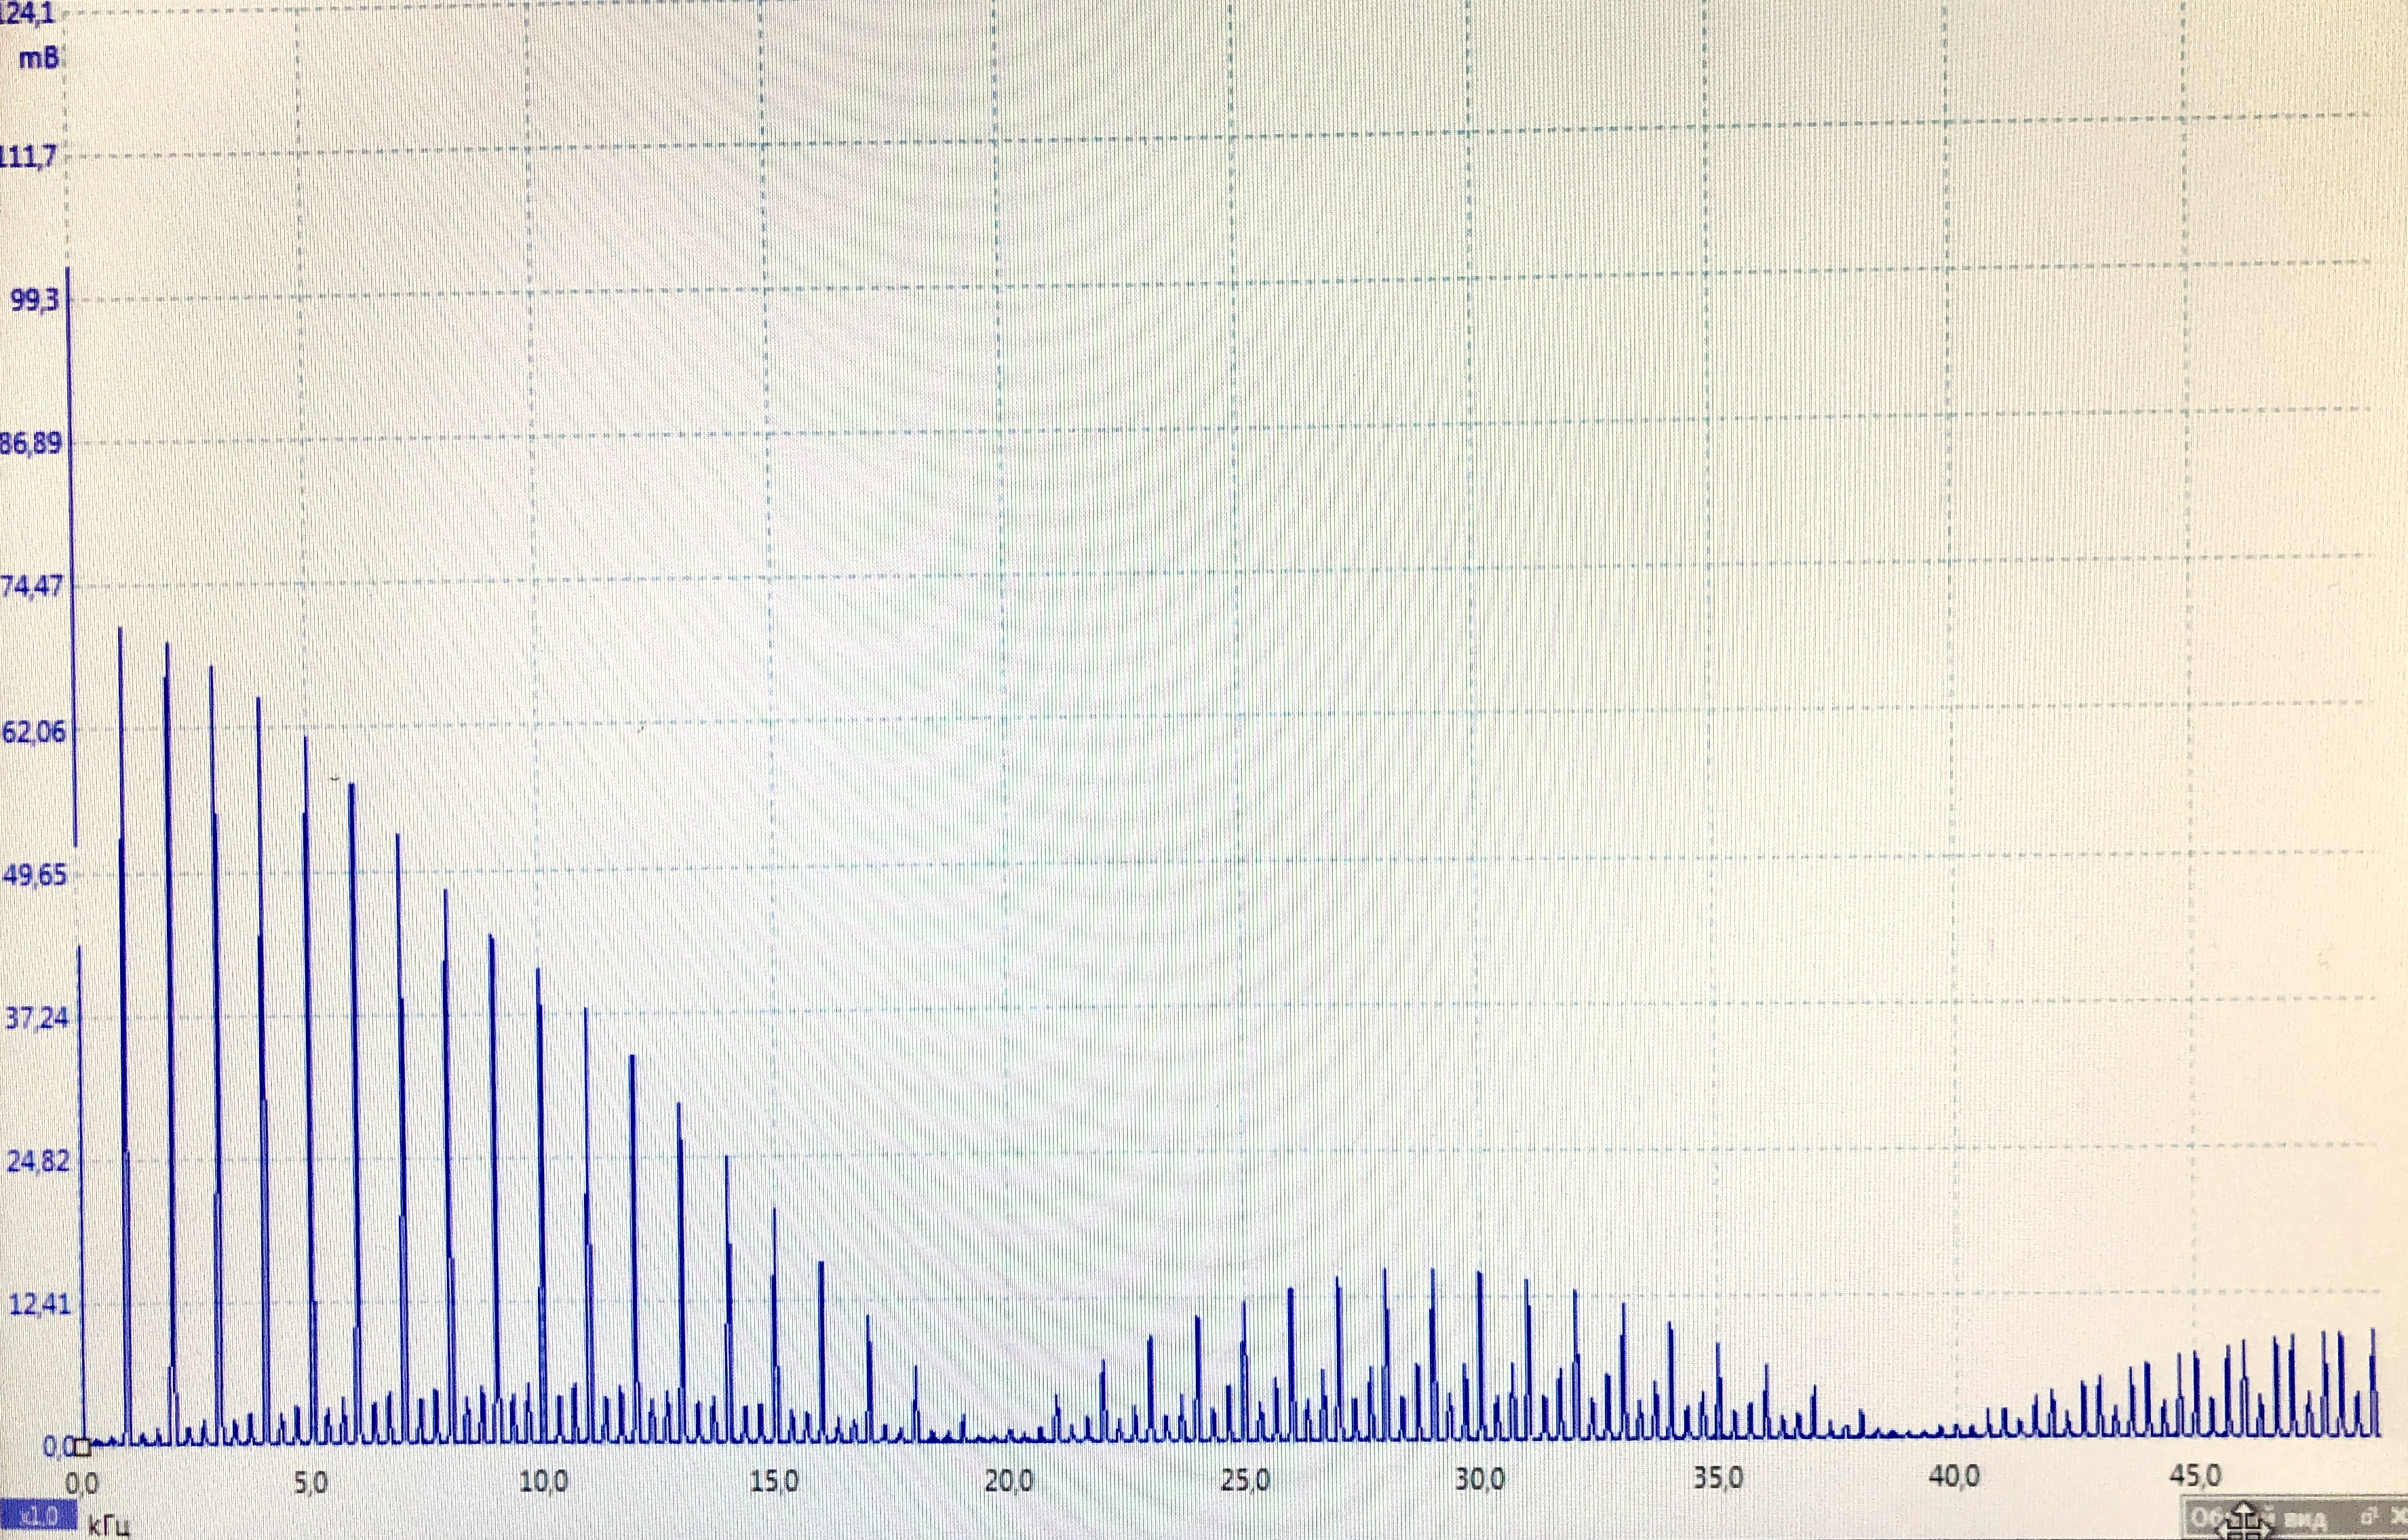
\includegraphics[width=0.4\linewidth]{1.png}
		\caption{Схема установки для изучения зависимости скорости звука от температуры}
	\end{figure}
	
Звуковые колебания в трубе возбуждаются телефоном Т и улавливаются микрофоном М. Мембрана телефона приводится в движение переменным током звуковой частоты. В качестве источника переменной ЭДС используется звуковой генератор ГЗ. Возникающий в микрофоне сигнал возникает на экране осциллографа ЭО.

Микрофон и телефон присоединены к установке через тонкие резиновые трубки. Такая связь достаточна для возбуждения и обнаружения звуковых колебаний в трубе и в то же время мало возмущает эти колебания: при расчетах оба конца трубы можно считать неподвижными, а влиянием соединительных отверстий пренебречь. 

Первая установка (рис. 1) содержит раздвижную трубу с миллиметровой шкалой. Через патрубок (на рисунке не показан) труба может наполняться воздухом или углекислым газом из газгольдера. На этой установке производятся измерения $\gamma$ для воздуха и для CO2. Вторая установка содерджит теплоизолированную трубу постоянной длины. Воздух в трубке нагревается водой из термостата.Температура газа принимается равной температуре омывающей трубу воды. 

\subsection*{Результаты измерений и обработка данных}
\subparagraph{1. Измерение скорости звука при помощи раздвижной трубы.}

\begin{enumerate}
    \item Исходя из примерного значения скорости звука $c=300$ м/c оценим диапозон частот, в котором необходимо вести измерения, чтобы можно было наблюдать 4 резонанса:
    \begin{equation*}
        \lambda = \frac {2 \Delta L_k}k,\ \Delta L \le 23\ см \Rightarrow \lambda \le 0.115\ м \Rightarrow f \ge 2600\ Гц.
    \end{equation*}
    \item Для углексилого газа будем снимать показания только при уменьшении длины, чтобы избежать попадания воздуха в трубку.
    \begin{center}
        \begin{tabular}{|c|c|c|c|c|c|c|c|c|}
            \hline
            f, Гц & \multicolumn{2}{|c|}{2498.8} &
            \multicolumn{2}{|c|}{4000.2} & \multicolumn{2}{|c|}{4503.4} & \multicolumn{2}{|c|}{3094.2}             
            \\
            \hline
             & $l_1$, см & $L_1$, см & $l_2$, см & $L_2$, см &$l_3$, см & $L_3$, см &$l_4$, см & $L_4$, см \\
            \hline
            &20.7 & 18.0 & 10.9 & 10.0 & 21.3 & 8.8 & 17.2 & 13.0 \\
            \hline
            &14.8 & 12.1 & 7.6 & 6.7 & 18.4 & 5.9 & 12.9 & 8.7 \\
            \hline
            &8.7 & 6.0 & 4.2 & 3.3 & 15.4 & 2.9 & 8.5 & 4.3 \\
            \hline 
            &2.7 & 0 & 0.9 & 0 & 12.5 & 0 & 4.2 & 0 \\
            \hline
        \end{tabular}
    \end{center}
    Здесь $l_k$ - значение на разметке трубы, $L_k$ - нормировка по минимальному значению.
    \item Изобразим полученные результаты на графике
\begin{figure*}[htp]
    \centering
    \includegraphics[width=0.5\linewidth]{CO2.png}
    \caption{График зависимости $L_k$ от k для $CO_2$}
    \label{fig:my_label}
\end{figure*}

Угловые коэффиценты получены методом наименьших квадратов:
\begin{equation*}
    k_\lambda = \frac{\langle L_k k \rangle}{\langle k^2\rangle},\ \sigma_k = \frac 1 {\sqrt n} \sqrt{\frac{\langle L_k^2 \rangle}{\langle k^2 \rangle}-k_\lambda^2}
\end{equation*}

Таким образом:
\begin{equation*}
    k_1 = 6.01\pm 0.02\ см, 
    k_2 = 3.34\pm 0.01\ см,
    k_3 = 2.94\pm 0.01\ см,
    k_4 = 4.34\pm 0.01\ см
\end{equation*}

Т.к. $k_\lambda=\frac{\lambda}{2},$ то из формулы (2) следует:
\begin{equation*}
    c_1 = 300.6\ м/c,\ 
    c_2 = 266.8\ м/c,\ 
    c_3 = 264.2\ м/c,\ 
    c_4 = 268.3\ м/c
    % c_1 = 300.6\pm 1.1\ м/c,
    % c_2 = 266.8\pm 0.9\ м/c,
    % c_3 = 264.2\pm 1.1\ м/c,
    % c_4 = 268.3\pm 0.8\ м/c
\end{equation*}

Отклонение значения, полученного в первом опыте можно объяснить плохим продувом трубки перед началом эксперимента (в трубке был воздух), поэтому учитывать его в расчетах не имеет смысла. 

\begin{equation*}
    c_{ср} = 266.43\ м/c,\ \sigma_{сл}=\sqrt{\frac{1}{n(n-1)}\sum^n_{i=1}(c_i-c_{ср})^2}
\approx 1.2\ м/c,\ \sigma_{сист} \ll \sigma_{сл}
\end{equation*}

Таким образом, полученная скорость распространения звука в углекислом газе равна $c=(266.4 \pm 1.2)\ м/c$.

По формуле (1) найдём $\gamma_{co_2}=C_p/C_v=1.270$ (Температура в помещении $22.6\pm0.1 ^o C$),
\begin{equation*}
    \sigma_\gamma=\sqrt{2\left(\frac{\sigma_c}{c}\right)^2+\left(\frac{\sigma_T}{T}\right)^2}\approx 0.006 \Rightarrow \gamma_{co_2}=1.270\pm0.006
\end{equation*}

\item Теперь аналогично проведем расчеты для воздуха. В ходе эксперимента выяснено, что данные при увеличении и уменьшении длины трубы отличаются несильно, поэтому можно использовать данные только при убывающей длине.

\begin{table}[ht!]
\begin{center}
\begin{tabular}{|c|cc|cc|cc|cc|}
\hline
f, Гц & \multicolumn{2}{c|}{1993.6}                & \multicolumn{2}{c|}{3100.0}                & \multicolumn{2}{c|}{3456.0}                & \multicolumn{2}{c|}{5017.0}                \\ \hline
      & \multicolumn{1}{l|}{$l_1$, см} & $L_1$, см & \multicolumn{1}{l|}{$l_2$, см} & $L_2$, см & \multicolumn{1}{l|}{$l_3$, см} & $L_3$, см & \multicolumn{1}{l|}{$l_4$, см} & $L_4$, см \\ \hline
      & \multicolumn{1}{l|}{21.1}      & 17.3      & \multicolumn{1}{l|}{21.7}      & 16.7      & \multicolumn{1}{l|}{22.9}      & 19.7      & \multicolumn{1}{l|}{22.5}      & 13.7      \\ \hline
      & \multicolumn{1}{l|}{12.4}      & 8.6       & \multicolumn{1}{l|}{16.2}      & 11.2      & \multicolumn{1}{l|}{18.0}      & 14.8      & \multicolumn{1}{l|}{17.1}      & 8.3       \\ \hline
      & \multicolumn{1}{l|}{3.8}       & 0         & \multicolumn{1}{l|}{10.6}      & 5.6       & \multicolumn{1}{l|}{13.0}      & 9.8       & \multicolumn{1}{l|}{15.7}      & 6.9       \\ \hline
      & \multicolumn{1}{l|}{}          &           & \multicolumn{1}{l|}{5.0}       & 0         & \multicolumn{1}{l|}{8.1}       & 4.9       & \multicolumn{1}{l|}{12.2}      & 3.4       \\ \hline
      & \multicolumn{1}{l|}{}          &           & \multicolumn{1}{l|}{}          &           & \multicolumn{1}{l|}{3.2}       & 0         & \multicolumn{1}{l|}{8.8}       & 0         \\ \hline
\end{tabular}
\end{center}
\end{table}

\begin{figure*}[htp]
    \centering
    \includegraphics[width=0.5\linewidth]{air.png}
    \caption{График зависимости $L_k$ от k для воздуха}
    \label{fig:my_label}
\end{figure*}

\begin{equation*}
    k_1 = 8.64\pm 0.02\ см, 
    k_2 = 5.58\pm 0.02\ см,
    k_3 = 4.92\pm 0.01\ см,
    k_4 = 3.23\pm 0.3\ см
\end{equation*}

\begin{equation*}
    c_1 = 344.5\ м/c,\ 
    c_2 = 345.9\ м/c,\ 
    c_3 = 340.3\ м/c,\ 
    c_4 = 324.1\ м/c
    % c_1 = 300.6\pm 1.1\ м/c,
    % c_2 = 266.8\pm 0.9\ м/c,
    % c_3 = 264.2\pm 1.1\ м/c,
    % c_4 = 268.3\pm 0.8\ м/c
\end{equation*}

\begin{equation*}
    c_{ср} = 338.7\ м/c,\ \sigma_{сл}=\sqrt{\frac{1}{n(n-1)}\sum^n_{i=1}(c_i-c_{ср})^2}
\approx 5.0\ м/c,\ \sigma_{сист} \ll \sigma_{сл}
\end{equation*}

Таким образом, полученная скорость распространения звука в воздухе равна $c=(338.7 \pm 5)\ м/c$.

По формуле (1) найдём $\gamma_{в}=C_p/C_v=1.35$,
\begin{equation*}
    \sigma_\gamma=\sqrt{2\left(\frac{\sigma_c}{c}\right)^2+\left(\frac{\sigma_T}{T}\right)^2}\approx 0.02 \Rightarrow \gamma_{в}=1.35\pm0.02
\end{equation*}
\end{enumerate}

\subparagraph{2. Изучение зависимости скорости звука от температуры.}
\begin{enumerate}
    \item Проведем теперь измерения и расчеты для второй установки.
    Длина трубы составляет $700\pm 1\ мм$.
    
    В таблице представлены значения полученных резонансных частот.
    
    \begin{table}[ht!]
    \begin{center}
        \begin{tabular}{|c|cc|cc|cc|cc|}
        \hline
        $t,^o C$ & \multicolumn{2}{c|}{22.6}                                        & \multicolumn{2}{c|}{38.8}                                        & \multicolumn{2}{c|}{44.0}                                        & \multicolumn{2}{c|}{54.0}                                        \\ \hline
        k        & \multicolumn{1}{l|}{$f_1,\ Гц \uparrow$} & $f_1,\ Гц \downarrow$ & \multicolumn{1}{l|}{$f_2,\ Гц \uparrow$} & $f_2,\ Гц \downarrow$ & \multicolumn{1}{l|}{$f_3,\ Гц \uparrow$} & $f_3,\ Гц \downarrow$ & \multicolumn{1}{l|}{$f_4,\ Гц \uparrow$} & $f_4,\ Гц \downarrow$ \\ \hline
        1        & \multicolumn{1}{l|}{263.70}              & 263.82                & \multicolumn{1}{l|}{273.62}              & 273.38                & \multicolumn{1}{l|}{277.46}              & 276.95                & \multicolumn{1}{l|}{280.25}              & 279.36                \\ \hline
        2        & \multicolumn{1}{l|}{498.11}              & 498.23                & \multicolumn{1}{l|}{509.00}              & 508.87                & \multicolumn{1}{l|}{512.58}              & 513.90                & \multicolumn{1}{l|}{521.85}              & 522.34                \\ \hline
        3        & \multicolumn{1}{l|}{738.81}              & 739.15                & \multicolumn{1}{l|}{758.20}              & 758.37                & \multicolumn{1}{l|}{767.51}              & 767.49                & \multicolumn{1}{l|}{774.00}              & 774.71                \\ \hline
        4        & \multicolumn{1}{l|}{987.55}              & 987.87                & \multicolumn{1}{l|}{1012.9}              & 1013.1                & \multicolumn{1}{l|}{1023.1}              & 1023.4                & \multicolumn{1}{l|}{1039.4}              & 1035.7                \\ \hline
        5        & \multicolumn{1}{l|}{1229.1}              & 1229.3                & \multicolumn{1}{l|}{1264.2}              & 1264.2                & \multicolumn{1}{l|}{1277.1}              & 1277.1                & \multicolumn{1}{l|}{1295.2}              & 1295.2                \\ \hline
    \end{tabular}
    \end{center}
\end{table}
Здесь стрелкой вверх обозначены резонансные частоты, полученные при повышении частоты, стрелкой вниз - при понижении.

Как видно, они отличаются несильно, что доказывает повторяемость результатов опыта. Для точности усредним полученные значения.

\begin{table}[htp]
\begin{center}
\begin{tabular}{|c|cc|cc|cc|cc|}
\hline
$t,^o C$ & \multicolumn{2}{c|}{22.6}                    & \multicolumn{2}{c|}{38.8}                    & \multicolumn{2}{c|}{44.0}                    & \multicolumn{2}{c|}{54.0}                    \\ \hline
k        & \multicolumn{1}{l|}{$f_1,\ Гц$} & $F_1,\ Гц$ & \multicolumn{1}{l|}{$f_2,\ Гц$} & $F_2,\ Гц$ & \multicolumn{1}{l|}{$f_3,\ Гц$} & $F_3,\ Гц$ & \multicolumn{1}{l|}{$f_4,\ Гц$} & $F_4,\ Гц$ \\ \hline
1        & \multicolumn{1}{l|}{263.76}     & 0          & \multicolumn{1}{l|}{273.50}     & 0          & \multicolumn{1}{l|}{277.21}     & 0          & \multicolumn{1}{l|}{279.81}     & 0          \\ \hline
2        & \multicolumn{1}{l|}{498.17}     & 234.41     & \multicolumn{1}{l|}{508.94}     & 235.44     & \multicolumn{1}{l|}{513.24}     & 236.03     & \multicolumn{1}{l|}{522.10}     & 242.29     \\ \hline
3        & \multicolumn{1}{l|}{738.98}     & 475.22     & \multicolumn{1}{l|}{758.29}     & 484.79     & \multicolumn{1}{l|}{767.50}     & 490.29     & \multicolumn{1}{l|}{774.36}     & 494.55     \\ \hline
4        & \multicolumn{1}{l|}{987.7}      & 723.9      & \multicolumn{1}{l|}{1013.0}     & 739.5      & \multicolumn{1}{l|}{1023.3}     & 746.1      & \multicolumn{1}{l|}{1037.6}     & 757.8      \\ \hline
5        & \multicolumn{1}{l|}{1229.2}     & 965.4      & \multicolumn{1}{l|}{1264.2}     & 990.7      & \multicolumn{1}{l|}{1277.1}     & 999.9      & \multicolumn{1}{l|}{1295.2}     & 1015.4     \\ \hline
\end{tabular}
\end{center}
\end{table}

Здесь $f_k$ - усредненное значение полученных частот, $F_k$ - нормированное значение по первой гармонике.

\item Построим график по полученным значениям (рис. 5) и занесем данные в таблицу.
\begin{figure}[h!]
    \centering
    \includegraphics[width=0.65\linewidth]{airT.png}
    \caption{График зависимости $F_k$ от k}
    \label{fig:my_label}
\end{figure}

По МНК:
\begin{equation*}
    k_1 = 240.6\pm 1.7\ Гц,\ k_2 = 246.2\pm2.6\ Гц,\ k_3 = 248.5\pm 2.8\ Гц,\ k_4 = 252.2\pm 2.8\ Гц
\end{equation*}

Из формулы (4) $c = 2Lk$.

% Из (1):
% \begin{equation*}
%     \gamma = \frac{\mu R}{T}c^2,\ 
%     \sigma_\gamma = \gamma \sqrt{2\left(\frac{\sigma_c}{c}\right)^2+\left(\frac{\sigma_T}{T}\right)^2}
% \end{equation*}

\begin{table}[ht!]
\begin{center}
\begin{tabular}{|c|c|c|c|c|c|c|c|}
\hline
$T, ^oC$ & $\sigma_T,\ ^oC$, & k, Гц & $\sigma_k$, Гц & $c$, м/c & $\sigma_c$, м/с & $\gamma$ & $\sigma_\gamma$ \\ \hline
22.6     & 0.1               & 240.6 & 1.7            & 336.8    & 2.4             & 1.34     & 0.12            \\ \hline
33.8     & 0.1               & 246.2 & 2.6            & 344.7    & 3.7             & 1.33     & 0.12            \\ \hline
44.0     & 0.1               & 248.5 & 2.8            & 347.9    & 3.9             & 1.33     & 0.12            \\ \hline
54.0     & 0.1               & 252.2 & 2.8            & 353.1    & 4.0             & 1.33     & 0.12            \\ \hline
\end{tabular}
\end{center}
\end{table}

Видно, что в рассматриваемом диапозане температур показатель адиабаты остается постоянным. Таким образом, усреднив значения, получаем $\gamma = 1.33\pm0.22$.
\end{enumerate}

\subsection*{Вывод}
В ходе выполнения работы были получены частоты и длины волн при резонансе звуковых колебаний в воздухе и углекислом газе. На основе полученных данных определены значения скорости распространения звука и показателей адиабат для указанных газов.

Для воздуха значения были получены двумя методами: при фиксированных частотах и переменной длине трубы, и при неизменной длине трубы, но различных температурах. Во втором эксперименте было определено, что в рассматриваемом диапазоне температур ($20^oC-60^oC$) показатель остается постоянным и равен $\gamma_{в_T}=1.33\pm0.22\ (\varepsilon \approx 15\%)$, что согласуется с числом, полученным первым методом $\gamma_{в_f}=1.35\pm0.02\ (\varepsilon \approx 2\%)$. Результат второго эксперимента в пределах погрешности совпадает с табличным $\gamma=1.4$, большая погрешность может быть объяснена большой чувствительностью ручки звукового генератора, в связи с чем определение момента резонанса может быть неточным. В первом эксперименте значение несильно отличается от табличного, что может быть связано с отличием температуры воздуха в трубке от комнатной (показатель адиабаты от температуры не зависит, но зависит скорость звука, по которой и проводился расчет).

Для углекислого газа значение было получено одним методом: при фиксированных частотах и переменной длине трубы. Во избежание попадания в трубку воздуха, измерения проводились только при убывающей длине трубы, после каждого опыта трубка заново продувалась углексилым газом. Полученное значение $\gamma_{co_2} = 1.270\pm0.006\ (\varepsilon \approx 1\%)$ несильно отличается от табличного $\gamma = 1.3$, что может быть связано с причиной, описанной для воздуха. Причину, связанную с возможным содержанием воздуха в трубке можно исключить, т.к. значение отличается от табличного в меньшую сторону, в то время как $\gamma_в=1.4>\gamma_{co_2}=1.3$.

\end{document}